\subsubsection{Domain-klasse: Settings}

Denne klasses formål er at gemme de nyeste data af hhv. bilens maksimale hastighed, kalibrering af styrtøj samt AKS status. Alle disse værdier har brugeren mulighed for at indstille fra PC'en. Disse data skal ligeledes være tilgængelige for andre klasser, der har brug for en eller flere af disse data. Da der arbejdes med mange threads i systemet, er det vigtigt at det ikke er muligt at skrive og læse fra de samme data af to forskellige threads på samme tid, til dette udnyttes mutex låse. På Figur \ref{fig:cd_settings} kan ses et klasse diagram over den ønskede klasse efterfulgt af funktionalitet.

\begin{figure}[h]
\centering
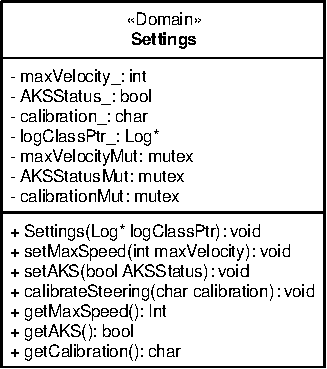
\includegraphics[]{../fig/diagrammer/bil/cd_settings.pdf}
\caption{Klassebeskrivelse for domain-klassen Settings}
\label{fig:cd_settings}
\end{figure}

\textbf{Attributter}

\begin{table}[h]
\begin{tabularx}{\textwidth}{| L{3cm} | Z | L{10cm} |} \hline
Navn & Type & Beskrivelse \\\hline
\texttt{maxVelocity\_}			& \texttt{int}		&Variabel af typen int til indhold af nuværende maksimal hastighed på bil.\\\hline

\texttt{AKSStauts\_}			& \texttt{bool}		&Variabel af typen bool til indhold af nuværende tilstand af AKS.\\\hline

\texttt{calibration\_}			& \texttt{char}		&Variabel af typen char der indeholder nuværende kalibrering til styrtøj.\\\hline

\texttt{logClassPtr\_}			& \texttt{Log*}		&En pointer til et object af typen Log. Gør det muligt at kalde funktioner fra Log objektet.\\\hline

\texttt{maxVelocitMut}			& \texttt{mutex}	&Mutex til kontrol af læsning og skrivning af/til maxVelocity\_ variabel fra flere threads.\\\hline

\texttt{AKSStautsMut}			& \texttt{mutex}	&Mutex til kontrol af læsning og skrivning af/til AKSStatus\_ variabel fra flere threads.\\\hline

\texttt{calibrationMut}			& \texttt{mutex}	&Mutex til kontrol af læsning og skrivning af/til calibration\_ variabel fra flere threads.\\\hline
\end{tabularx}
\caption{Attributter for klassen Settings}
\label{table:attr_settings}
\end{table}

\clearpage

\textbf{Metoder}

\begin{table}[h]
\begin{tabularx}{\textwidth}{| L{2.5 cm} | Z |} \hline
Prototype 	& \texttt{void Settings(Log* logClassPtr)} \\\hline
Parametre 	& \texttt{logClassPtr} 		\newline En pointer til objektet af typen Log der bruges til at lave en association til objektet. \\\hline
Beskrivelse	& Constructor til klassen Settings. \newline \\\hline
\end{tabularx}
\caption{Metodebeskrivelse for constructoren af \texttt{Settings} klassen}
\label{table:met_settings}
\end{table}

\begin{table}[h]
\begin{tabularx}{\textwidth}{| L{2.5 cm} | Z |} \hline
Prototype 	& \texttt{void setMaxSpeed(int maxVelocity)} \\\hline
Parametre 	& \texttt{maxVelocity}		\newline Den hastighed der ønskes sættet til maksimal hastighed for bil.\\\hline
Returværdi	& \texttt{void} 			\newline \\\hline
Beskrivelse	& Denne funktion har til formål at skrive til variablen maxVelocity\_. \newline \\\hline
\end{tabularx}
\caption{Metodebeskrivelse for \texttt{setMaxSpeed()}}
\label{table:met_setmaxspeed}
\end{table}

\begin{table}[h]
\begin{tabularx}{\textwidth}{| L{2.5 cm} | Z |} \hline
Prototype 	& \texttt{void setAKS(bool AKSStatus)} \\\hline
Parametre 	& \texttt{AKSStatus}		\newline Den ønskede tilstand af AKS status for bil.\\\hline
Returværdi	& \texttt{void} 			\newline \\\hline
Beskrivelse	& Denne funktion har til formål at skrive til variablen AKSStatus\_.\newline \\\hline
\end{tabularx}
\caption{Metodebeskrivelse for \texttt{setAKS()}}
\label{table:met_setaks}
\end{table}

\begin{table}[h]
\begin{tabularx}{\textwidth}{| L{2.5 cm} | Z |} \hline
Prototype 	& \texttt{void calibrateSteering(char calibration)} \\\hline
Parametre 	& \texttt{calibration}		\newline Den ønskede kalibrering af bilens styrtøj.\\\hline
Returværdi	& \texttt{void} 			\newline \\\hline
Beskrivelse	& Denne funktion har til formål at skrive til variablen calibration\_.\newline \\\hline
\end{tabularx}
\caption{Metodebeskrivelse for \texttt{calibratesteering()}}
\label{table:met_calibratesteering}
\end{table}

\clearpage

\begin{table}[h]
\begin{tabularx}{\textwidth}{| L{2.5 cm} | Z |} \hline
Prototype 	& \texttt{int getMaxSpeed()} \\\hline
Parametre 	& \texttt{void}			\newline \\\hline
Returværdi	& \texttt{int} 			\newline Returnerer variablen maxVelocity\_\\\hline
Beskrivelse	& Denne funktion har til formål at give muligheden for at læse variablen maxVelocity\_.\newline \\\hline
\end{tabularx}
\caption{Metodebeskrivelse for \texttt{getMaxSpeed()}}
\label{table:met_getmaxspeed}
\end{table}

\begin{table}[h]
\begin{tabularx}{\textwidth}{| L{2.5 cm} | Z |} \hline
Prototype 	& \texttt{bool getAKS()} \\\hline
Parametre 	& \texttt{void}			\newline \\\hline
Returværdi	& \texttt{bool}			\newline Returnerer variablen AKSStatus\_\\\hline
Beskrivelse	& Denne funktion har til formål at give muligheden for at læse variablen AKSStatus\_.\newline \\\hline
\end{tabularx}
\caption{Metodebeskrivelse for \texttt{getAKS()}}
\label{table:met_getaks}
\end{table}

\begin{table}[h]
\begin{tabularx}{\textwidth}{| L{2.5 cm} | Z |} \hline
Prototype 	& \texttt{char getCalibration()} \\\hline
Parametre 	& \texttt{void}			\newline \\\hline
Returværdi	& \texttt{char} 		\newline Returnerer variablen calibration\_\\\hline
Beskrivelse	& Denne funktion har til formål at give muligheden for at læse variablen calibration\_.\newline \\\hline
\end{tabularx}
\caption{Metodebeskrivelse for \texttt{getCalibration()}}
\label{table:met_getcalibration}
\end{table}